%Analysis
\section{Internet of Value and Blockchain}
\label{sec:analysis}

When the Internet was created, it had a simple goal: connect computers so they could share data reliably, even if parts of the network failed.
As the technology matured, the goal shifted towards enabling people to communicate by computer and transfer data through the World Wide Web.
Anyone could spin up a simple Apache server at home and distribute HTML files over the web using the Hypertext Transfer Protocol (HTTP).
However, most pages were still static, stateless content. For many internet users, the experience was novel because they could use email and access the latest news without waiting until the next day for a printed paper.
In 1996, when CSS1.0 was introduced in browsers, we could customize the web page's design to our preferences \cite{Choudhury2014}.

Several early e-commerce applications were also created, including Amazon.com.
This era is commonly called Web 1.0 or the Internet of Information. The web consisted mainly of pages accessible from any browser.
Powered by speculation in new startups, Web 1.0 ended in the dot-com era \cite{Goodnight2010}.
Large numbers of users joined during the Web 2.0 era. Although Web 2.0 did not depend on one single technological breakthrough, it changed how people used the web.

Web pages became more interactive thanks to JavaScript and frameworks such as jQuery. Web 2.0 mainly uses HTML5 and CSS3, and its defining feature is that the web became social and interconnected.
The distinctive shift in Web 2.0 was that non-technical users could create and share content online, from a blog post on WordPress to a YouTube video \cite{Web1, Krumm2008, Chakravorty2017}.
With the first release of Facebook in 2004, the web became a place where information spread more easily and quickly.
These platforms allowed non-technical people to create blogs and websites.

The Internet also enabled the sharing economy. Instead of owning a car, users can rent one and pay only for the time they use it \cite{Parker2016}.
Most vehicles are used only 5\% of the day \cite{Keith2022}, which means that they are heavily underutilized. A similar pattern appears in housing.
Before the Internet, people mostly rented houses or flats to friends or family members. The Internet lowered transaction costs and made it easier to share assets with strangers.
Platforms like Airbnb were created to make the renting process more accessible. We do not need to limit the platform economy\footnote{Commonly known as the gig economy.} only to asset sharing \cite{Cupi2022, Sundararajan2016}.
TaskRabbit allowed people to sell their time for specific tasks \cite{Prassl2015}.
The problem is that people participating in the platform economy must earn a reputation for each service separately.
For example, we can have an impressive reputation score in TaskRabbit, but if we want to become Airbnb hosts, we must build our reputation again \cite{Schor2016}.
Web 2.0 moved information and access online but kept settlement, ownership, and reputation locked inside individual operators. The Internet of Value is the paradigm that sets out to remove that limit, and the rest of this chapter examines where it has succeeded, where it has not, and what is missing.

As described in Chapter~\ref{sec:blockchain}, blockchain technology provides the foundational infrastructure for decentralized, trustless value transfer through consensus-driven state transitions \cite{Nakamoto, wood2014ethereum}. Building on these primitives, the decentralized finance (DeFi) sector has demonstrated that traditional financial products, such as lending (Compound \cite{papangelou2023exploring}, AAVE \cite{gambacorta2024defi, frangella2022aave}), decentralized exchange (Uniswap \cite{Adams2021}), and asset management, can be replicated in a permissionless, composable manner \cite{Angeris2020, Kim2022}.

The emergence of blockchain technology enabled a shift from an Internet of Information to an Internet of Value. While the former revolutionized how we share and access data, the latter promises
to transform how we transfer, store, and exchange assets of any kind.
However, the term Internet of Value is often conflated with related but distinct concepts. ``Web3'' broadly refers to the decentralized web stack (identity, storage, computation), while ``decentralized finance'' denotes the specific application of blockchain to financial instruments. The Internet of Value is a broader paradigm: it encompasses not only financial transactions but any form of value transfer, including non-monetary assets such as reputation, access rights, intellectual property, and governance participation.

Lohmer et al. \cite{Lohmer2024} define the Internet of Value as follows:

\begin{quote}
The Internet of Value enables the direct transfer of assets of any kind as well as processing and settlement of business transactions based on blockchain technology in conjunction with digital platforms, tokens, smart contracts, and other technologies such as the Internet of Things and artificial intelligence. Its principles are to create a system compliant with data protection values, equal and fair access for all participants, effective representation of digital and physical assets, and disintermediation for direct peer-to-peer communication and the exchange of values. These technologies and principles facilitate open content and value sharing, transparency, sustainable behavior, and self-sovereign digital identities \cite{Lohmer2024}.
\end{quote}

From the definition, we can derive three essential elements that differentiate the Internet of Value from previous paradigms.
First, blockchain is treated as the foundation of the IoV rather than as just one supporting technology. Secure value transfer requires orchestration among multiple participants in the network, which leads to the second element: the Internet of Value as a fair and autonomous socio-economic framework rather than merely a technical infrastructure.

Third, the definition implies that value itself is not a singular, objective quantity but a multi-dimensional construct. Through expert interviews and systematic analysis, Lohmer et al. \cite{Lohmer2024} later summarized this understanding to propose that value in the Internet of Value can be defined using three distinct dimensions: Economic worth, Utility or access rights, and Ethical and sustainability contributions.

The remainder of this chapter argues that the distance between this definition and what current platforms actually deliver is best read as three analytical gaps: multidimensional value, agent-compatible policy boundaries, and scalable governance evaluation. Figure \ref{fig:three-gaps} summarises these gaps and points to ICVP as the response.

\begin{figure}[H]
    \centering
    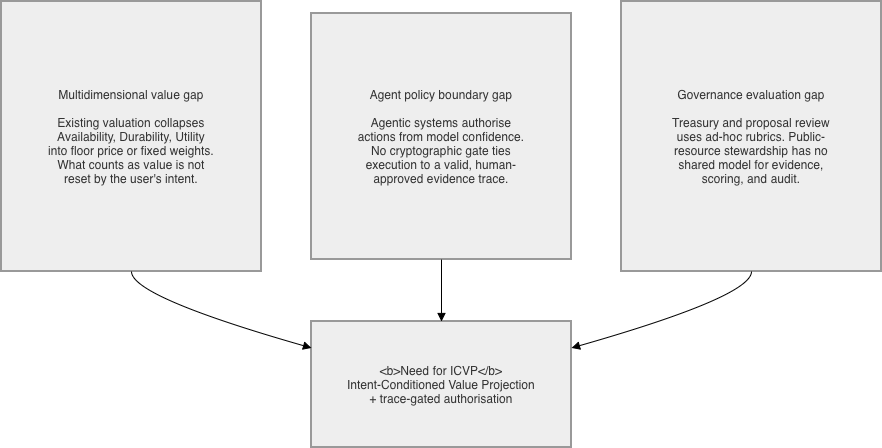
\includegraphics[width=0.85\columnwidth,height=0.72\textheight,keepaspectratio]{images/three-gaps.png}
    \caption{Three analytical gaps that motivate Intent-Conditioned Value Projection.}
    \label{fig:three-gaps}
\end{figure}

The first gap follows from the multi-dimensional reading above: asset valuation in the Internet of Value cannot rest on price discovery alone. Non-fungible tokens can have a low floor market price yet carry high utility for a specific community \cite{Ante2021, Dowling2022, Nadini2021, Kong2021}. Fungible governance tokens can be cheap to obtain yet contribute meaningfully to on-chain decision-making. Traditional financial valuation frameworks that prioritize market price and liquidity fail to capture this. The absence of a multi-dimensional valuation framework that captures utility and contribution alongside price is the first analytical gap this thesis addresses, and it is taken up formally in Chapter~\ref{sec:aims}.

The second gap concerns the boundary at which a semi-autonomous agent is allowed to act. Blockchain provides the infrastructure for storing and sharing data without trusted intermediaries, and through tokenization any asset can be represented on-chain with verifiable ownership and transferability \cite{Jeon2022}. This eliminates the risk that a centralised operator pulls the asset offline by shutting down its servers \cite{Duan2021}, and it makes assets across the network tradeable, lockable as collateral, and composable with other protocols \cite{Williams2019, Gudgeon2020}. In multi-chain ecosystems this composability also extends to non-fungible assets, whose ownership and utility may need to move across parachain boundaries rather than remain tied to one ledger \cite{Morhac2024nftsharing}. As the Internet of Value expands across multiple chains and absorbs an ever-growing diversity of asset shapes, from tokenised real-world assets and generative algorithms to blockchain-native protocols and intellectual property rights \cite{Bambridge2022}, the action space available to a programmatic actor grows accordingly. The problem is that current account models do not provide policy boundaries that this actor can be safely operated within. Externally owned accounts bind authority to a single key. Smart contract wallets, including recent account-abstraction proposals such as EIP-4337 \cite{Buterin2021, Wang2023, Duan2024}, focus on flexible authentication and gas sponsorship rather than agent-oriented delegation. None of them expose primitives for policy enforcement, risk isolation, and audit-trace-gated decision-making that stay compatible with existing DeFi protocols. The agentic literature has shown that large language models can plan and call tools \cite{Sumers2024, Wu2023, Wang2024survey}, and the user-centric AI literature has long argued that delegation requires the user to remain aware of and able to override ongoing actions \cite{Amershi2019, Shneiderman2022, Wang2021}. Neither concern is met by an account model that treats every signed transaction as equally authoritative. The lack of agent-compatible policy boundaries at the account level is the second analytical gap this thesis addresses.

The third gap concerns governance at scale. Open-source projects and public goods cannot be funded by manual case-by-case assessment once volume rises \cite{Kukelka2022public, Calhoun2006, Ostrom1990}. Open-source code itself creates value, both by allowing multiple parties to contribute to the same codebase, which makes the project more stable and less prone to bugs \cite{Sopko2022}, and by letting non-technical contributors propose ideas and improvements \cite{Alves2022, Yin2021}. Two on-chain mechanisms have emerged to fund this work. Quadratic funding gives backers skin in the game and lets matchers amplify support for shared goals \cite{Buterin2018QF, Buterin2019, Pasquini2021, Buterin2018, Freitas2021, Weyl2018}. On-chain treasury proposals route funding through community votes, with the project receiving funds if the proposal passes \cite{Rodrigues2022, Valastin2024proto}. Both mechanisms require processing on-chain and off-chain evidence about spending history, deliverables, and ecosystem fit, and at realistic volumes this evaluation cost is the binding constraint. Polkadot's OpenGov system processes hundreds of proposals per year, each one requiring analysis of on-chain spending history, team track records, deliverable feasibility, and alignment with ecosystem priorities \cite{Valastin2024proto}. Individual voters lack the time and tooling to do this consistently, which leads to voter apathy, low participation rates, and decisions driven by social influence rather than evidence. The framing this thesis takes is that agentic systems act as a decision-support layer that retrieves evidence, structures it across multiple dimensions, and produces auditable recommendations for human voters \cite{Wang2024survey}. Final voting authority stays with human participants or formally authorised governance actors. Blockchain stays the settlement layer that records approved actions in a transparent and immutable form. The two layers are complementary, not substitutes. The agent does not replace human judgement, and the chain does not interpret value. The scalability limit on manual governance evaluation is the third analytical gap this thesis addresses.

Despite the literature on blockchain-based asset valuation \cite{DeLope2021}, no standardized framework yet exists for multi-dimensional, goal-oriented asset valuation, account models do not yet expose the policy boundaries a semi-autonomous agent needs, and governance still assumes voters can keep up with proposal volume. These three gaps, the absence of a multi-dimensional valuation framework, the lack of agent-compatible policy boundaries at the account level, and the scalability limit on manual governance evaluation, motivate the research questions formulated in Chapter~\ref{sec:aims}.
